\chapter{Implementação}
\label{cap5}



Este capítulo visa expressar o funcionamento prático dos microsserviços implementados.
%
Isto é necessário pois as escolhas técnicas, envolvendo as linguagens adotadas, as tecnologias utilizadas e boas práticas aplicadas no desenvolvimento das aplicações, interferem na qualidade dos microsserviços.
%
Denotando-se qualidade como o consumo de recursos e desempenho das aplicações.





Devido as diversas possibilidades de linguagens de programação e bibliotecas disponíveis, a Seção~\ref{sec:tecnologias} tem o objetivo de descrever as tecnologias utilizadas para o desenvolvimento das aplicações e justificar tais escolhas.
%
Além disso, a Seção~\ref{sec:tecnologias} apresenta o conjunto de serviços externos utilizados para facilitar o desenvolvimento dos microsserviços.
%
O serviços externos apesar de não estarem diretamente implementados na arquitetura das soluções, foram utilizados durante o processo e devem ser evidenciados.



Diante da complexidade das arquiteturas de microsserviços desenvolvidos, torna-se necessário descrever quais microsserviços foram implementados, e como estão dispostos na rede.
%
Para este fim, a Seção~\ref{sec:interconexao} contextualiza a interconexão dos microsserviços desenvolvidos.



\section{Tecnologias Utilizadas}
\label{sec:tecnologias}



A seleção das tecnologias e bibliotecas que são executadas nas aplicações é importante, visto que elas implicam diretamente no desempenho e consumo de recursos das arquiteturas selecionadas.
%
Entretanto, essa seleção precisa estar de acordo com as regras de negócio impostas para os testes.



Inicialmente, existe uma preocupação com a linguagem de programação utilizada, visto que ela precisa ter um bom desempenho, um suporte a programação paralela e, ao mesmo tempo, conter bibliotecas que auxiliem no desenvolvimento ágil de tais serviços.
%
Neste sentido, foi levantado um conjunto de linguagens de programação, o qual viabilize o projeto de acordo com os seguintes critérios:



\begin{itemize}
  \item Alto desempenho para programas paralelos;
  \item Biblioteca para conexão com banco de dados PostgreSql;
  \item Biblioteca para uso de cache (Redis);
  \item Biblioteca para escrita de serviços \ac{rpc}, sobre o protocolo \ac{tcp};
  \item Biblioteca para escrita de serviços \textit{web}, com \ac{api} no formato \ac{json};
  \item Linguagem compilada;
  \item Linguagem com tipagem estática; e
  \item Simplicidade de escrita de código, preferencialmente.
\end{itemize}



A partir destes critérios, a linguagem selecionada foi a linguagem GoLang, por se tratar de uma linguagem a qual o autor possui domínio e satisfaz os critérios definidos anteriormente.



Outro critério, o qual é implícito para o desenvolvimento, é a homogenidade da linguagem de programação em todos os microsserviços.
%
Tal necessidade gera o benefício da escrita de código reutilizável, como o núcleo de regras de negócio que pode ser aplicado a todas as arquiteturas desenvolvidas.



Desta forma, foi selecionada uma única linguagem de desempenho compatível com a viabilização do projeto.
%
Em função da diversidade de bibliotecas disponíveis, também é necessário definir quais bibliotecas foram utilizadas para o desenvolvimento das arquiteturas dos microsserviços.
%
Dentre as bibliotecas utilizadas, destacam-se:



\begin{itemize}
  \item gin: Servidor Web para serviços de alto desempenho;
  \item gorm: Biblioteca de objetos relacionais, a qual suporta conexão direta ao banco PostgreSQL;
  \item go-redis: Biblioteca para conexão ao serviço Redis;
  \item net/rpc: Biblioteca nativa da linguagem GoLang para escrita de serviços \ac{rpc} sobre o protocolo \ac{tcp};
  \item graphite: Biblioteca de conexão ao banco de métricas;
  \item testify: Biblioteca auxiliar a suíte nativa de testes da linguagem.
\end{itemize}



Tais bibliotecas foram utilizadas na camada de infraestrutura, sendo seu uso aplicado a todas as arquiteturas.
%
A camada de infraestrutura é responsável pela realização da interação entre a rede e as regras de negócio dos microsserviços.


Destaca-se, dentre as bibliotecas citadas, a biblioteca testify.
%
Tal biblioteca foi utilizada na garantia de integridade das aplicações desenvolvidas.
%
Sua finalidade é realizar a inspeção automatizada do funcionamento da aplicação.
%
Entretanto, a biblioteca não é utilizada durante a execução da aplicação, denotando-se como uma biblioteca auxiliar.



As bibliotecas auxiliares foram utilizadas no processo de integração contínua.
%
O processo de integração contínua foi implantado utilizando os serviços externos Github e TravisCI.
%
Este processo é descrito como processo de construção na arquitetura Willson, sendo responsável pelo teste e envio de imagens de contêineres a um serviço de resgistro na nuvem.




Após descrever as tecnologias utilizadas, faz-se necessário descrever o ambiente distribuído desenvolvido, a fim de garantir uma melhor visibilidade dos microsserviços implementados.



\section{Interconexão entre os microsserviços}
\label{sec:interconexao}



A interconexão entre os microsserviços refere-se ao projeto de rede de uma arquitetura qualquer, disponilizando visualmente a camada de rede.
%
Ao todo foram implementados onze microsserviços, os quais possuem a qual comunicam-se por troca de mensagens.
%
Tais conexões entre sí, com os bancos de dados e com os seus respectivos clientes foram definidas pelos autores das arquiteturas.
%
Consequentemente, torna-se interessante descrever a interconexão entre os microsserviços, exibindo assim seus protocolos de comunicação de rede.



A arquitetura Rudy contém um microsserviço intermediário para conexão com o banco de dados.
%
Esta disposição de microsserviços está exposto na Subseção~\ref{sec:inter_rudy}.



A arquitetura Salz remove a responsabilidade de mensageria do jogo do microsserviço de jogo.
%
Outra alteração é a exposição do microsserviço de autenticação como uma interface pública na rede, permitindo a conexão a partir dos clientes.
%
Esta disposição de microsserviços da arquitetura Salz é descrito na Subseção~\ref{sec:inter_salz}.



A arquitetura Willson tem o funcionamento semelhante a arquitetura Rudy, porém não utiliza um microsserviço intermediário para organização de consultas ao banco de dados.
%
A disposição dos microsserviços nesta arquitetura é visível na Subseção~\ref{sec:inter_willson}.



\subsection{Rudy}
\label{sec:inter_rudy}


A arquitetura Rudy em versão reduzida para o escopo dos testes contém quatro microsserviços e dois banco de dados, sendo um para dados permanentes (PostgreSQL) e um para cache (Redis).
%
Os seus microsserviços estão listados na Tabela~\ref{tab:inter_rudy}.

\begin{table}[htb!]
\centering
\begin{adjustbox}{max width=\textwidth}
\caption{Microsserviços da arquitetura Rudy.}
\label{tab:inter_rudy}
\begin{tabular}{l|l|l}
\hline
Nome            & Protocolo            & Público a Rede \\ \hline
 rgame          & \ac{rpc}/\ac{tcp}    & \checkmark     \\ \hline
 rweb           & \ac{http}/\ac{json}  & \checkmark     \\ \hline
 rauth          & \ac{rpc}/\ac{tcp}    &                \\ \hline
 rcrud          & \ac{rpc}/\ac{tcp}    &                \\ \hline
\end{tabular}
\end{adjustbox}

Fonte: O próprio autor.
\end{table}



Os microsserviços da arquitetura Rudy, descritos na Tabela~\ref{tab:inter_rudy}, possuem funcionalidades próprias.
%
A funcionalidade de cada microsserviço é:



\begin{itemize}
  \item \textit{rgame}: Este microsserviço é responsável por gerenciar o posicionamento dos personagens, execução das operações do mundo e troca de mensagens do chat do jogo. Ele também é responsável por autenticar contas ao mundo do jogo.
  \item \textit{rweb}: Este microsserviço é responsável por receber requisições web como uma \ac{api} a fim de criar novas contas e novos personagens para o jogo.
  \item \textit{rauth}: Este microsserviço é responsável por autenticar e garantir uma única conexão por conta em determinada arquitetura.
  \item \textit{rcrud}: Este microsserviço é responsável por realizar o acesso ao banco de dados, retornando os dados da consulta a qual é requisitada.
\end{itemize}



Dado tais características, temos um ponto de atenção no microsserviço \textit{rcrud} a qual cria uma barreira de acesso ao banco de dados.
%
Este padrão de projeto tende a facilitar a manutenção do banco de dados, centralizando tipos de requisições.
%
O seu objetivo é mover o escopo de consulta a dados em um ponto centralizado, evitando falhas ao armazenar e obter tais dados.
%
Este processo é escalável, entretanto adiciona uma camada maior ao obter os dados, na qual tende a aumentar o tempo de resposta para as operações ao banco.
%
A disposição da arquitetura Rudy está visível na Figura~\ref{fig:interconexao_rudy}.



\begin{figure}[htb!]
  \caption{Interconexões da arquitetura Rudy.}
  \label{fig:interconexao_rudy}
  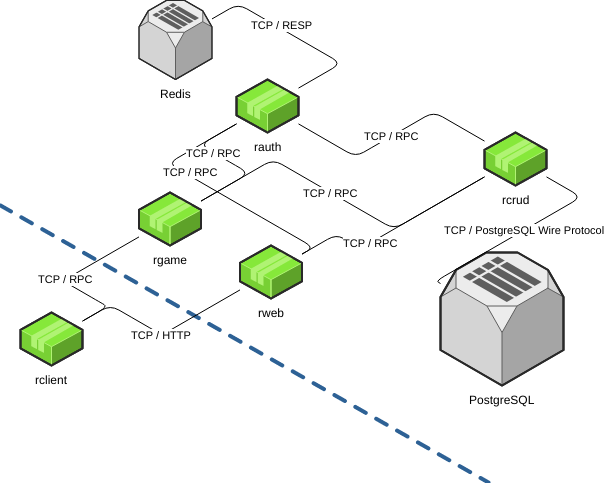
\includegraphics[width=0.8\textwidth]{figuras/interconexoes/rudy.png}
  \centering

  Fonte: O próprio autor.
\end{figure}



Outro ponto de atenção é o acesso ao microsserviço de autenticação \textit{rauth}, a qual pode ser visualizado na Figura~\ref{fig:interconexao_rudy}.
%
Tal microsserviço é privado, dessa forma o microsserviço de mundo fica responsável em ser um ponto intermediário de comunicação entre o cliente e o serviço que realmente realiza a autenticação.
%
Este padrão de projeto é comum em aplicações Web, entretanto não recomendado pelo padrão sujerido a utilização do \ac{jwt}.



O padrão \ac{jwt} recomenda tornar o microsserviço de autenticação público, na qual o cliente realiza a autenticação direta com o microsserviço de autenticação, reduzindo tráfego interno de rede.
%
Mesmo não sendo um padrão recomendado, tal característica não deve ter um impácto significativo para arquiteturas de jogos \ac{mmorpg}, visto que esta operação é realizada poucas vezes no serviço.



Entretanto, a arquitetura Salz realiza alterações compatíveis com o padrão \ac{jwt} e remove microsserviços privados, usando uma interconexão de microsserviços plana.
%
Dessa forma, torna-se de interesse descrever tais características a fim de permitir comparações na arquitetura.



\subsection{Salz}
\label{sec:inter_salz}



A arquitetura Salz em versão reduzida para o escopo dos testes contém quatro microsserviços e dois banco de dados, sendo um para dados permanentes (PostgreSQL) e um para cache (Redis).
%
Os seus microsserviços estão listados na Tabela~\ref{tab:inter_salz}.



\begin{table}[htb!]
\centering
\begin{adjustbox}{max width=\textwidth}
\caption{Microsserviços da arquitetura Salz.}
\label{tab:inter_salz}
\begin{tabular}{l|l|l}
\hline
Nome            & Protocolo            & Público a Rede \\ \hline
 sgame          & \ac{rpc}/\ac{tcp}    & \checkmark     \\ \hline
 schat          & \ac{rpc}/\ac{tcp}    & \checkmark     \\ \hline
 sweb           & \ac{http}/\ac{json}  & \checkmark     \\ \hline
 sauth          & \ac{rpc}/\ac{tcp}    & \checkmark     \\ \hline
\end{tabular}
\end{adjustbox}

Fonte: O próprio autor.
\end{table}



Os microsserviços da arquitetura Salz, descritos na Tabela~\ref{tab:inter_salz}, possuem funcionalidades próprias.
%
A funcionalidade de cada microsserviço é:



\begin{itemize}
  \item \textit{sgame}: Este microsserviço é responsável por gerenciar o posicionamento dos personagens, execução das operações do mundo e troca de mensagens do chat do jogo.
  \item \textit{schat}: Este microsserviço é responsável por gerenciar mensagens entre jogadores, porém possui um forte aclopamento com o microsserviço \textit{sgame}.
  \item \textit{sweb}: Este microsserviço é responsável por receber requisições web como uma \ac{api} a fim de criar novas contas e novos personagens para o jogo.
  \item \textit{sauth}: Este microsserviço é responsável por autenticar e garantir uma única conexão por conta em determinada arquitetura.
\end{itemize}



Dado tais características, damos atenção ao microsserviço \textit{schat}.
%
Tal microsserviço é responsável por gerenciar todo o serviço de chat da arquitetura, seja baseado em região de interesse ou global.
%
Entretanto a informação de posicionamento não está armazenada neste microsserviço.
%
Nesse sentido, esta característica obriga um custo de sincronização destes dados, que implica diretamente em custo de recurso ou tempo de resposta para o cliente.
%
A topologia pode ser visualizada na Figura~\ref{fig:interconexao_salz}.



\begin{figure}[htb!]
  \caption{Interconexões da arquitetura Salz.}
  \label{fig:interconexao_salz}
  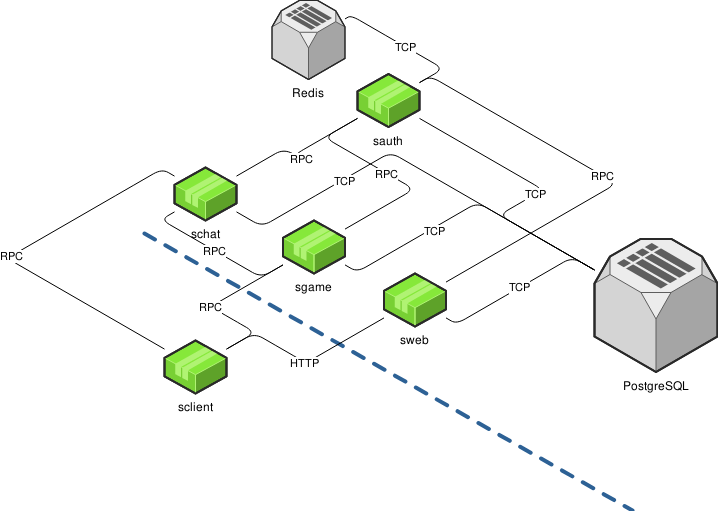
\includegraphics[width=0.8\textwidth]{figuras/interconexoes/salz.png}
  \centering

  Fonte: O próprio autor.
\end{figure}



Outra característica desta arquitetura é a comunicação direta entre o microsserviço de autenticação \textit{sauth} e o cliente.
%
Isto evita uma conexão intermediária utilizando o microsserviço \textit{sgame}, na qual permite maior vasão de dados sobre autenticação e sessão.
%
Outro ponto a ser ressaltado é a possibilidade de utilizar \ac{jwt} para autenticação, sem a necessidade de verificação pelo próprio microsserviço de autenticação.



Tal característica da interconexão da arquitetura Salz torna o sistema de autenticação independente, permitindo adicionar novos serviços de forma flexível.
%
Também pode-se notar uma possível utilização de verificação de sessão por assinatura digital, validando uma assinatura do microsserviço de autenticação, diminuindo o consumo da rede para mensagens de verificação pelo serviço de autenticação.



Entretanto, não foi utilizado tal método de validação de sessão.
%
O método atual consiste em validação de assinatura utilizando o banco de dados de cache.
%
De tal forma, obriga-se a comunicação entre os microsserviços \textit{schat} e \textit{sgame} com o microsserviço \textit{sauth}.
%
Esta escolha foi realizada para manter os mesmos métodos de autenticação em todas as arquiteturas, evitando variação por algoritmos ou tecnologia.



Dado tais características da arquitetura Salz, a sincronização de posições entre o microsserviço \textit{schat} e \textit{sgame} pode ser um problema conforme a frequência da sincronização necessária pela regra de negócio do jogo implementado.
%
Dessa forma, a arquitetura Willson propõe um ponto intermediário entre as arquiteturas Salz e Rudy, tornando-se interessante descrever suas alterações.



\subsection{Willson}
\label{sec:inter_willson}


A arquitetura Willson em versão reduzida para o escopo dos testes contém três microsserviços e dois banco de dados, sendo um para dados permanentes (PostgreSQL) e um para cache (Redis).
%
Os seus microsserviços estão listados na Tabela~\ref{tab:inter_willson}.



\begin{table}[htb!]
\centering
\begin{adjustbox}{max width=\textwidth}
\caption{Microsserviços da arquitetura Willson.}
\label{tab:inter_willson}
\begin{tabular}{l|l|l}
\hline
Nome            & Protocolo            & Público a Rede \\ \hline
 wweb           & \ac{http}/\ac{json}  & \checkmark     \\ \hline
 wgame          & \ac{rpc}/\ac{tcp}    & \checkmark     \\ \hline
 wauth          & \ac{rpc}/\ac{tcp}    &                \\ \hline
\end{tabular}
\end{adjustbox}

Fonte: O próprio autor.
\end{table}


Os microsserviços da arquitetura Willson, descritos na Tabela~\ref{tab:inter_willson}, possuem funcionalidades próprias.
%
A funcionalidade de cada microsserviço é:



\begin{itemize}
  \item \textit{wgame}: Este microsserviço é responsável por gerenciar o posicionamento dos personagens, execução das operações do mundo e troca de mensagens do chat do jogo. Ele também gerencia a sessão do jogador, tendo um forte aclopamento com o microsserviço \textit{wauth}.
  \item \textit{wweb}: Este microsserviço é responsável por receber requisições web como uma \ac{api} a fim de criar novas contas e novos personagens para o jogo.
  \item \textit{wauth}: Este microsserviço é responsável por autenticar e garantir uma única conexão por conta em determinada arquitetura.
\end{itemize}



Dado os microsserviços da arquitetura Willson, listados na Tabela~\ref{tab:inter_willson}, uma característica interessante é a auxência de um microsserviço de gerencia de mensagens de chat e um intermediário para gestão de dados do banco.
%
Estas características tornam a arquitetura mais simples, dividindo os microsserviços em domínios específicos em pontos que necessitam de escalabilidade.
%
A interconexão da arquitetura Willson pode ser visualizada na Figura~\ref{fig:interconexao_willson}.


\begin{figure}[htb!]
  \caption{Interconexões da arquitetura Willson.}
  \label{fig:interconexao_willson}
  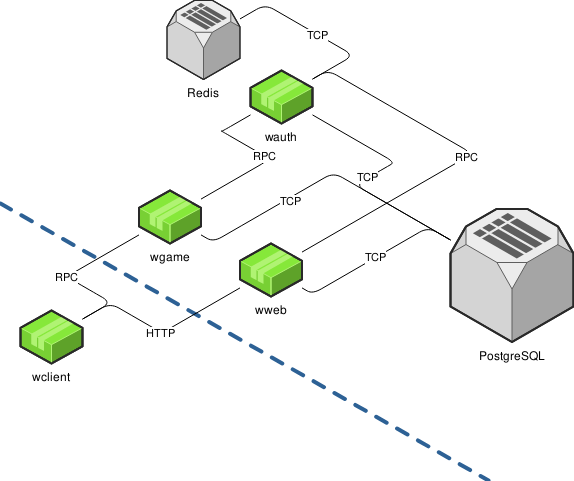
\includegraphics[width=0.8\textwidth]{figuras/interconexoes/willson.png}
  \centering

  Fonte: O próprio autor.
\end{figure}
